% Auto-generated by _refactor_rendu.py
\clearpage
\section*{Figures}
\addcontentsline{toc}{section}{Figures}
\setcounter{figure}{0}

\begin{figure}[H]
\centering

\includegraphics[width=\linewidth]{duopoly_vs_triopoly.png}
\caption{Duopoly vs.\ triopoly equilibrium.}
\label{fig:duopoly-vs-triopoly}
\end{figure}

\begin{figure}[H]
\centering

\includegraphics[width=\linewidth]{quantity_comparison.png}
\caption{Quantity comparison across structures.}
\label{fig:quantity-comparison}
\end{figure}

\begin{figure}[H]
\centering

\includegraphics[width=\linewidth]{profit_comparison.png}
\caption{Profit comparison across structures.}
\label{fig:profit-comparison}
\end{figure}

\begin{figure}[H]
\centering

\includegraphics[width=\linewidth]{comparative_statics.png}
\caption{Comparative statics on the demand intercept.}
\label{fig:comparative-statics}
\end{figure}

\begin{figure}[H]
\centering

\includegraphics[width=\linewidth]{market_power.png}
\caption{Market-power metrics: Lerner indices and HHI across market
structures.}
\label{fig:market-power}
\end{figure}

\begin{figure}[H]
\centering

\includegraphics[width=\linewidth]{stackelberg_comparison.png}
\caption{Stackelberg comparison: first-mover premium by leader.}
\label{fig:stackelberg-comparison}
\end{figure}

\begin{figure}[H]
\centering

\includegraphics[width=\linewidth]{capacity_constrained_vs_unconstrained.png}
\caption{Constrained versus unconstrained equilibria at calibrated
capacities ($\mathrm{cap}_{\text{US}} = 30$,
$\mathrm{cap}_{\text{OPEC}} = 40$, $\mathrm{cap}_{\text{RUS}} = 35$~mbd).}
\label{fig:capacity-constrained}
\end{figure}

\begin{figure}[H]
\centering

\includegraphics[width=\linewidth]{capacity_binding_analysis.png}
\caption{Capacity binding analysis: identification of the binding player
at Nash and at cartel quotas.}
\label{fig:capacity-binding}
\end{figure}

\begin{figure}[H]
\centering

\includegraphics[width=\linewidth]{capacity_opec_sweep.png}
\caption{OPEC capacity sweep: equilibrium price, output, and per-player
profit as $\mathrm{cap}_{\text{OPEC}}$ varies from $25$ to $60$~mbd.}
\label{fig:capacity-opec-sweep}
\end{figure}

\begin{figure}[H]
\centering

\includegraphics[width=\linewidth]{capacity_folk_theorem.png}
\caption{Capacity and the Folk Theorem: critical discount factor
$\delta^\ast$ as a function of OPEC capacity.}
\label{fig:capacity-folk-theorem}
\end{figure}

\begin{figure}[H]
\centering

\includegraphics[width=\linewidth]{welfare_decomposition.png}
\caption{Welfare decomposition across the six benchmark market
structures: competitive, Nash, Stackelberg by leader, and cartel.}
\label{fig:welfare-decomposition}
\end{figure}

\begin{figure}[H]
\centering

\includegraphics[width=\linewidth]{welfare_dwl_comparison.png}
\caption{Deadweight loss comparison across market structures, ranking
from competitive ($0$) to cartel ($1{,}800$).}
\label{fig:welfare-dwl}
\end{figure}

\begin{figure}[H]
\centering

\includegraphics[width=\linewidth]{welfare_carbon_tax.png}
\caption{Carbon tax interaction: collusion premium as a function of
per-barrel Pigouvian tax $\tau \in \{0,10,20,30,40,50\}$.}
\label{fig:welfare-carbon-tax}
\end{figure}

\begin{figure}[H]
\centering

\includegraphics[width=\linewidth]{welfare_surplus_distribution.png}
\caption{Surplus distribution: consumer surplus, producer surplus by
player, and deadweight loss across market structures.}
\label{fig:welfare-surplus}
\end{figure}

\begin{figure}[H]
\centering

\includegraphics[width=\linewidth]{bertrand_nash_equilibrium.png}
\caption{Differentiated Bertrand-Nash equilibrium at $\sigma = 0.6$.}
\label{fig:bertrand-nash}
\end{figure}

\begin{figure}[H]
\centering

\includegraphics[width=\linewidth]{bertrand_vs_cournot.png}
\caption{Cournot versus Bertrand: side-by-side comparison of prices,
quantities, profits, and consumer surplus.}
\label{fig:bertrand-vs-cournot}
\end{figure}

\begin{figure}[H]
\centering

\includegraphics[width=\linewidth]{bertrand_sigma_sweep.png}
\caption{Substitutability sweep: equilibrium quantities as $\sigma$
varies from $0$ to $1$; convergence toward marginal-cost pricing.}
\label{fig:bertrand-sigma-sweep}
\end{figure}

\begin{figure}[H]
\centering

\includegraphics[width=\linewidth]{bertrand_cooperation_gap.png}
\caption{Cooperation gap under differentiated Bertrand: average price
under Bertrand-Nash versus cooperative Bertrand.}
\label{fig:bertrand-cooperation-gap}
\end{figure}

\begin{figure}[H]
\centering

\includegraphics[width=\linewidth]{repeated_dynamics_combined.png}
\caption{Repeated-game myopic best-response: prices, total quantity,
per-player quantities, and per-player profits converging to the static
Nash benchmark at $\lambda = 0.2$.}
\label{fig:repeated-dynamics-combined}
\end{figure}

\begin{figure}[H]
\centering

\includegraphics[width=\linewidth]{convergence_after_shock.png}
\caption{Convergence after a large adverse demand shock: mean recovery
path with $80$~percent confidence band.}
\label{fig:convergence-after-shock}
\end{figure}

\begin{figure}[H]
\centering

\includegraphics[width=\linewidth]{lambda_sensitivity.png}
\caption{$\lambda$-sensitivity analysis of myopic best-response dynamics:
monotone convergence for $\lambda \in (0, 0.5)$, oscillatory for
$\lambda \in (0.5, 1)$.}
\label{fig:lambda-sensitivity}
\end{figure}

\begin{figure}[H]
\centering

\includegraphics[width=\linewidth]{repeated_punishment_regimes.png}
\caption{Punishment regime simulation: cooperate, deviate, be punished,
recover.}
\label{fig:repeated-punishment}
\end{figure}

\begin{figure}[H]
\centering

\includegraphics[width=\linewidth]{folk_theorem.png}
\caption{Folk Theorem: critical discount factors $\delta_i^\ast$ by
player.}
\label{fig:folk-theorem}
\end{figure}

\begin{figure}[H]
\centering

\includegraphics[width=\linewidth]{correlated_eq_comparison.png}
\caption{Correlated equilibrium versus Nash and cartel: price and
per-player profit for the three CE objectives (max-welfare,
max-joint-profit, max-min).}
\label{fig:ce-comparison}
\end{figure}

\begin{figure}[H]
\centering

\includegraphics[width=\linewidth]{correlated_eq_support_all.png}
\caption{Support of the correlated equilibrium: action profiles
recommended by the mediator and their probability weights, across the
three objectives.}
\label{fig:ce-support}
\end{figure}

\begin{figure}[H]
\centering

\includegraphics[width=\linewidth]{correlated_eq_welfare.png}
\caption{Welfare ranking of the three correlated equilibria against
Nash and cartel benchmarks.}
\label{fig:ce-welfare}
\end{figure}

\begin{figure}[H]
\centering

\includegraphics[width=\linewidth]{shapley_values.png}
\caption{Shapley value decomposition for the OPEC--US--Russia triopoly.}
\label{fig:shapley}
\end{figure}

\begin{figure}[H]
\centering

\includegraphics[width=\linewidth]{green_porter_regimes.png}
\caption{Green--Porter cooperation regimes under $AR(1)$ and
jump-diffusion demand.}
\label{fig:green-porter-regimes}
\end{figure}

\begin{figure}[H]
\centering

\includegraphics[width=\linewidth]{green_porter_coop_survival.png}
\caption{Green--Porter cooperation survival probabilities across shock
specifications.}
\label{fig:green-porter-survival}
\end{figure}

\begin{figure}[H]
\centering

\includegraphics[width=\linewidth]{delta_star_comparison.png}
\caption{Critical discount factor $\delta^\ast$ under deterministic and
stochastic demand: side-by-side comparison.}
\label{fig:delta-star-comparison}
\end{figure}

\begin{figure}[H]
\centering

\includegraphics[width=\linewidth]{stochastic_price_bands.png}
\caption{Monte Carlo price bands (P10, median, P90) under $AR(1)$
demand shocks.}
\label{fig:stochastic-price-bands}
\end{figure}

\begin{figure}[H]
\centering

\includegraphics[width=\linewidth]{stochastic_jump_diffusion.png}
\caption{\citet{merton1976} jump-diffusion demand specification:
simulated price paths with rare discrete jumps.}
\label{fig:stochastic-jump-diffusion}
\end{figure}

\begin{figure}[H]
\centering

\includegraphics[width=\linewidth]{stochastic_comparison.png}
\caption{Deterministic versus stochastic equilibrium: distribution of
terminal price across $300$ Monte Carlo paths.}
\label{fig:stochastic-comparison}
\end{figure}

\begin{figure}[H]
\centering

\includegraphics[width=\linewidth]{demand_shock_scenarios.png}
\caption{Demand shock scenarios: equilibrium price, output, and
per-player profit at $\delta_a \in \{-30, -20, -10, 0, +10, +20, +30\}$.}
\label{fig:demand-shock-scenarios}
\end{figure}

\begin{figure}[H]
\centering

\includegraphics[width=\linewidth]{evo_payoff_matrix.png}
\caption{Evolutionary game theory: stage-game payoff matrix for the
Cooperate, Defect, and Punish strategies.}
\label{fig:evo-payoff-matrix}
\end{figure}

\begin{figure}[H]
\centering

\includegraphics[width=\linewidth]{evo_phase_2strategy.png}
\caption{Two-strategy replicator dynamics (Cooperate vs.\ Defect): phase
line and ESS.}
\label{fig:evo-phase-2strategy}
\end{figure}

\begin{figure}[H]
\centering

\includegraphics[width=\linewidth]{evo_phase_3strategy.png}
\caption{Three-strategy replicator dynamics (Cooperate, Defect, Punish):
triangular phase diagram showing bistability.}
\label{fig:evo-phase-3strategy}
\end{figure}

\begin{figure}[H]
\centering

\includegraphics[width=\linewidth]{evo_punishment_sweep.png}
\caption{Punishment-severity sensitivity sweep: long-run population
composition as a function of the punishment multiplier.}
\label{fig:evo-punishment-sweep}
\end{figure}

\begin{figure}[H]
  \centering
  
\includegraphics[width=\linewidth]{figures/policy_heatmaps.png}
  \caption{Greedy-policy heatmaps for the three learning agents
           on a representative headline seed. Colour encodes
           the greedy output action (mbd); blank cells were
           never visited during training. The absence of any
           systematic price-quantity gradient corroborates the
           Spearman finding of
           Section~\ref{subsec:reciprocity}: converged policies
           are largely unresponsive to the observed price,
           consistent with path-dependent fixed-point lock-in.}
  \label{fig:heatmaps}
\end{figure}
\begin{figure}[H]
  \centering
  
\includegraphics[width=\linewidth]{figures/basins_histogram.png}
  \caption{Per-seed distribution of the greedy collusion index
           in the headline triopoly ($n = 50$ seeds, top) and
           duopoly robustness check ($n = 50$ seeds, bottom).
           The bimodal structure of the triopoly distribution
           motivates the Wilson-proportion reformulation of
           Section~\ref{subsec:basins}: the appropriate summary
           is the proportion of seeds reaching a cooperative
           basin ($\CI \geq 0.20$), not the cross-seed mean.
           The duopoly distribution collapses to a tight
           predatory cluster, confirming the regime contrast
           documented in Section~\ref{subsec:duopoly}.}
  \label{fig:basins}
\end{figure}
\begin{figure}[H]
  \centering
  
\includegraphics[width=0.92\linewidth]{ci_caterpillar.png}
  \caption{Collusion index across all Section~4 regimes: point
           estimate and $95\%$ confidence interval (Wilson or
           normal-approximation as reported in the corresponding
           table), anchored to $\CI = 0$ (static Nash) and
           $\CI = 1$ (joint-profit cartel). Single-learner and
           duopoly regimes sit in predatory territory below Nash;
           every multi-learner and robustness regime sits in the
           cooperative half-space. The coarse-grid point carries no
           reported interval.}
  \label{fig:ci-forest}
\end{figure}

\clearpage
\section*{Tables}
\addcontentsline{toc}{section}{Tables}
\setcounter{table}{0}

\begin{table}[H]
\centering
\caption{Green-Porter steady-state statistics under $AR(1)$ and
jump-diffusion demand shocks.}
\label{tab:green-porter}
\renewcommand{\arraystretch}{1.2}
\small
\begin{tabular}{lcc}
\toprule
\textbf{Statistic} & \textbf{$AR(1)$ shocks} & \textbf{Jump-diffusion} \\
\midrule
Cooperation fraction & 94\,\% & 85\,\% \\
Mean cooperative spell & $61.8$ qtrs ($\sim$15 yrs) & $39.1$ qtrs ($\sim$10 yrs) \\
Mean punishment phase & $9.6$ qtrs ($\sim$2.4 yrs) & $9.5$ qtrs ($\sim$2.4 yrs) \\
Triggers ($300$ paths $\times\,200$ qtrs) & $291$ & $685$ \\
\bottomrule
\end{tabular}
\end{table}

\begin{table}[H]
  \centering
  \caption{Headline triopoly: central statistics across
           $50$ independent seeds. The greedy estimator freezes
           Q-tables and sets $\varepsilon = 0$; the tail
           estimator averages the final $20\%$ of training
           at $\varepsilon = 0.05$. The gap between the two is
           a diagnostic of residual exploration at the end of
           training.}
  \label{tab:headline}
  \small
  \begin{tabular}{lcccc}
    \toprule
    Estimator
      & Mean $\CI$
      & Std.\ dev.\
      & $95\%$ CI (mean)
      & Mean $\bar{P}$ (\$/bbl) \\
    \midrule
    Tail of training & 0.61 & 0.18 & $[0.57,\;0.67]$ & 68.41 \\
    Greedy rollout   & 0.73 & 0.39 & $[0.62,\;0.84]$ & 72.63 \\
    \midrule
    Random policy (baseline) & 0.04 & --- & $[-0.04,\;0.12]$ & 44.20 \\
    \bottomrule
  \end{tabular}
\end{table}
\begin{table}[H]
  \centering
  \caption{Basin classification of the $50$ headline seeds by
           greedy collusion index. Seed counts and share of
           total are reported for each qualitatively distinct
           attractor.}
  \label{tab:basins}
  \small
  \begin{tabular}{lccl}
    \toprule
    Basin & Greedy $\CI$ range & Seeds ($n$) & Qualitative label \\
    \midrule
    Predatory    & $\CI < 0$         &  3 & Below-Nash pricing \\
    Competitive  & $0 \le \CI < 0.20$&  0 & Near-Nash \\
    Cooperative  & $0.20 \le \CI < 0.80$ & 12 & Tacit cooperation \\
    Near-cartel  & $\CI \ge 0.80$    & 35 & Supra-cooperative \\
    \bottomrule
  \end{tabular}
\end{table}
\begin{table}[H]
  \centering
  \caption{Wilson score intervals for the proportion of seeds
           reaching a cooperative basin ($\CI \geq 0.20$),
           by regime and estimator. Non-overlapping intervals
           imply a strict separation between triopoly and
           duopoly at the $5\%$ level.}
  \label{tab:wilson}
  \small
  \begin{tabular}{lcc}
    \toprule
    Regime
      & $\hat{p}\;(\CI \geq 0.20)$
      & Wilson $95\%$ interval \\
    \midrule
    Triopoly (greedy)    & 0.94 & $[0.84,\;0.98]$ \\
    Triopoly (tail)      & 0.88 & $[0.76,\;0.95]$ \\
    Duopoly  (greedy)    & 0.00 & $[0.00,\;0.07]$ \\
    Duopoly  (tail)      & 0.02 & $[0.00,\;0.11]$ \\
    \bottomrule
  \end{tabular}
\end{table}
\begin{table}[H]
  \centering
  \caption{Forced-deviation experiment: multi-seed mean price
           and per-player quantities in each window
           ($n = 20$ seeds). The strategic share is computed
           via Equation~\eqref{eq:strategic}.}
  \label{tab:forced}
  \small
  \begin{tabular}{lccccc}
    \toprule
    Window
      & $\bar{P}$ (\$/bbl)
      & $\bar{q}_{\text{OPEC}}$ (mbd)
      & $\bar{q}_{\text{US}}$ (mbd)
      & $\bar{q}_{\text{RUS}}$ (mbd)
      & $\bar{Q}$ (mbd) \\
    \midrule
    Pre-window  & 79.75 & 24.98 & 16.92 & 18.35 & 60.25 \\
    During      & 64.15 & 38.57 & 18.10 & 19.17 & 75.84 \\
    Post-window & 78.92 & 25.31 & 17.05 & 18.40 & 60.76 \\
    \midrule
    $\Delta$ (during $-$ pre) & $-15.60$ & $+13.59$ & $+1.18$ & $+0.82$ & $+15.59$ \\
    \bottomrule
  \end{tabular}
\end{table}
\begin{table}[H]
  \centering
  \caption{Punishment-cycle detection: per-seed results at
           the full headline budget ($75{,}000$ steps,
           $n = 5$ seeds). The pre-registered frequency band
           is $[0.2,\,2.0]$ cycles per $1{,}000$ steps.}
  \label{tab:cycles}
  \small
  \begin{tabular}{lcccl}
    \toprule
    Seed
      & Cycles detected
      & Freq.\ (per $1{,}000$ steps)
      & Median drop (\$/bbl)
      & In band? \\
    \midrule
    301 & 289 & 3.85 & 12.14 & No \\
    302 &  84 & 1.12 & 11.02 & \textbf{Yes} \\
    303 &  34 & 0.45 & 10.87 & \textbf{Yes} \\
    304 & 255 & 3.40 & 11.93 & No \\
    305 & 291 & 3.88 & 11.89 & No \\
    \midrule
    Median & --- & --- & 11.57 & $2/5$ \\
    \bottomrule
  \end{tabular}
\end{table}
\begin{table}[H]
  \centering
  \caption{Policy-level Spearman $\rho$ between greedy output
           action and price bin, by seed and agent
           ($n = 5$ seeds, full headline budget).}
  \label{tab:spearman-policy}
  \small
  \begin{tabular}{lcccc}
    \toprule
    Seed & OPEC & US & RUS & Row median \\
    \midrule
    301 &  0.04 &  0.01 & $-0.02$ &  0.01 \\
    302 &  0.07 &  0.03 &  0.01   &  0.03 \\
    303 & $-0.01$ & 0.05 & 0.02   &  0.02 \\
    304 &  0.02 & $-0.03$ & 0.04  &  0.02 \\
    305 &  0.06 &  0.00 &  0.01   &  0.01 \\
    \midrule
    Column median & 0.04 & 0.01 & 0.01 & \textbf{0.02} \\
    \bottomrule
  \end{tabular}
\end{table}
\begin{table}[H]
  \centering
  \caption{Realised-trajectory Spearman $\rho$ between price
           at step $t$ and agent output at step $t+1$,
           post-convergence window ($n = 5$ seeds).}
  \label{tab:spearman-real}
  \small
  \begin{tabular}{lcccc}
    \toprule
    Seed & OPEC & US & RUS & Row median \\
    \midrule
    301 &  0.11 &  0.06 &  0.04 &  0.06 \\
    302 &  0.14 &  0.09 & $-0.03$ & 0.09 \\
    303 &  0.03 &  0.08 &  0.10 &  0.08 \\
    304 &  0.05 & $-0.02$ & 0.12 & 0.05 \\
    305 &  0.09 &  0.07 &  0.06 &  0.07 \\
    \midrule
    Column median & 0.09 & 0.07 & 0.06 & \textbf{0.07} \\
    \bottomrule
  \end{tabular}
\end{table}
\begin{table}[H]
  \centering
  \caption{Demand-shock experiment: window-level scalars
           aggregated across $20$ observations ($10$ seeds
           $\times\,2$ shocks). $\sigma_P$ is computed from
           the pre-shock rolling window.}
  \label{tab:shocks}
  \small
  \begin{tabular}{lcc}
    \toprule
    Diagnostic & Median & Pre-registered threshold \\
    \midrule
    In-window mean drop ($\sigma_P$ units) & 2.73 & $\geq 2.00$ \\
    Trough drop ($\sigma_P$ units)         & 5.78 & --- \\
    Recovery half-life (steps)             &   11 & $\leq 15{,}000$ \\
    Post-shock converged $\CI$             & 0.96 & --- \\
    \bottomrule
  \end{tabular}
\end{table}
\begin{table}[H]
  \centering
  \caption{Verdict matrix: all eight pre-registered
           decision rules applied verbatim to the Option~B
           evidence. Secondary hypotheses Q5--Q8 denote the
           robustness checks of
           Section~\ref{subsec:robustness}. \protect\badgelegend}
  \label{tab:matrix}
  \small
  \begin{tabular}{llcc}
    \toprule
    Label & Pre-registered criterion & Verdict & Section \\
    \midrule
    H1 & Greedy $\CI$ lower bound $\geq 0.30$
        & \vyes~\textbf{Met}     & \ref{subsec:headline} \\
    H2 & Learner-count ordering, non-overlapping CIs
        & \vyes~\textbf{Met}     & \ref{subsec:learners} \\
    H3 & Spearman $\rho(\gamma,\CI) > 0$, disjoint extremes
        & \vyes~\textbf{Met}     & \ref{subsec:gamma} \\
    H4a & Strategic share $\geq 30\%$
        & \vno~\textbf{Not met} & \ref{subsec:forced} \\
    H4b & Cycle frequency in $[0.2,\,2.0]$, $\geq 3/5$ seeds
        & \vno~\textbf{Not met} & \ref{subsec:cycles} \\
    H4c & Spearman median $\rho \geq 0.30$
        & \vno~\textbf{Not met} & \ref{subsec:reciprocity} \\
    H5  & Leader quantity within $\pm 20\%$ of $q_L^\ast$
        & \vpart~\textbf{Partial} & \ref{subsec:stack} \\
    \midrule
    Q6  & Cap on/off: CIs non-overlapping
        & \vpart~Not met (sweep: \textbf{Met}) & \ref{subsec:cap} \\
    Q7  & $\alpha$-sweep: greedy CI $> 0.30$ at all cells
        & \vyes~\textbf{Met}     & \ref{subsec:alpha} \\
    Q8  & Shock recovery within $4\times$ shock width
        & \vyes~\textbf{Met}     & \ref{subsec:shocks} \\
    \bottomrule
  \end{tabular}
\end{table}
\begin{table}[H]
  \centering
  \caption{Cross-model ranking of market structures from the
           most competitive (lowest $\bar{P}$) to the most
           collusive (highest $\bar{P}$). All prices are in
           $\$\text{/bbl}$; the corresponding collusion index
           is reported in the final column.}
  \label{tab:synth-rank}
  \small
  \begin{tabular}{llccc}
    \toprule
    Rank & Market structure & $\bar{P}$ & $\CI$ & Section \\
    \midrule
    1 & Perfect competition           & 35.0 & $-$  & 2.1 \\
    2 & Single Q-learner (predatory)  & 56.3 & $-0.19$ & \ref{subsec:learners} \\
    3 & Cournot--Nash                 & 60.0 & 0.00 & 2.2 \\
    4 & Correlated equilibrium        & 66.4 & 0.32 & 3.3 \\
    5 & MARL triopoly (greedy)        & 72.6 & 0.73 & \ref{subsec:headline} \\
    6 & Cartel (joint-profit max.)    & 80.0 & 1.00 & 3.2 \\
    \bottomrule
  \end{tabular}
\end{table}

\clearpage
\appendix


\section{Calibrated parameters of the linear-Cournot triopoly}
\label{app:calibration}

\small
\setlength{\tabcolsep}{4pt}
\renewcommand{\arraystretch}{1.15}
\begin{longtable}{@{}>{\raggedright\arraybackslash}p{0.19\linewidth} c c
  >{\raggedright\arraybackslash}p{0.46\linewidth}@{}}
\caption*{Calibrated parameters of the linear-Cournot triopoly, grouped
by analytical block. Each row reports the parameter, its symbol, its
calibrated value, and the rationale and source linking the value to the
empirical literature or to a deliberate modelling choice.}
\label{tab:calibration} \\
\toprule
\textbf{Parameter} & \textbf{Symbol} & \textbf{Value} & \textbf{Rationale and source} \\
\midrule
\endfirsthead
\caption*{(continued) Calibrated parameters of the linear-Cournot triopoly} \\
\toprule
\textbf{Parameter} & \textbf{Symbol} & \textbf{Value} & \textbf{Rationale and source} \\
\midrule
\endhead
\midrule
\multicolumn{4}{r}{\small(continued on next page)} \\
\endfoot
\bottomrule
\endlastfoot
\multicolumn{4}{l}{\emph{A. Demand}}\\
\midrule
Demand intercept & $a$ & \$140/bbl & Choke price at upper end of
\citealp{iea2019} WEO long-run scenarios; implies monopoly $P$ of \$80, within
Saudi fiscal break-even range (IMF Article IV). \\
Demand slope & $b$ & $1.0$ & Normalisation. Implies own-price elasticity
of approx.\ $-0.75$ at triopoly Nash, mid-range of EIA Short-Term
Energy Outlook ($-0.4$ to $-1.0$) and \citet{hamilton2003}. \\
\midrule
\multicolumn{4}{l}{\emph{B. Marginal costs (short-run, well-level, per barrel)}}\\
\midrule
OPEC marginal cost & $c_{\text{OPEC}}$ & \$20 & Gulf wellhead lifting
($\sim$\$5-\$10, \citealp{bp2022}) plus transport, infrastructure and
fiscal overhead. Consistent with Aramco Q1 2026 disclosed cost.
\emph{Not} the fiscal break-even of \$80. \\
Russia marginal cost & $c_{\text{RUS}}$ & \$35 & Siberian lifting
($\sim$\$15-\$20, \citealp{imf2021}), Urals export differential
($\sim$\$10-\$15), plus $\sim$\$5 sanctions premium. \\
US shale cost & $c_{\text{US}}$ & \$45 & Well-level break-even
(Dallas Fed Energy Survey, 2020). Firm-level Permian break-even
(\$61-\$62 in Q1 2025 survey) embeds corporate overhead, outside
short-run Cournot best-response margin. \\
\midrule
\multicolumn{4}{l}{\emph{C. Capacities (mbd)}}\\
\midrule
OPEC capacity & $\mathrm{cap}_{\text{OPEC}}$ & $40$ & Sum of sustainable
capacity of OPEC core (OPEC MOMR, 2024-2026 avg). Set at unconstrained
Nash output to make binding at Nash and slack at cartel. \\
Russia capacity & $\mathrm{cap}_{\text{RUS}}$ & $35$ & Upper bound on
non-OPEC OPEC+ bloc expansion under existing infrastructure
(\citealp[p.~??]{henderson2015}; \citealp{eia2025}). \\
US capacity & $\mathrm{cap}_{\text{US}}$ & $30$ & Upper bound for US
shale consistent with Permian Wolfcamp tier estimates (\citealp{smith2016};
EIA Permian assessment). \\
OPEC capacity sweep & & $25$-$60$ & Range spans 2022-23 tight regime
and 2020 slack regime; brackets all empirically observed levels. \\
\midrule
\multicolumn{4}{l}{\emph{D. Time and patience}}\\
\midrule
Discount factor & $\delta$ & $0.95$ & Quarterly frequency matching
OPEC+ meeting cadence. Annualised $\sim$19\%, deliberately elevated to
proxy political and fiscal impatience. Comfortably above binding
$\delta_{\text{OPEC}}^\ast = 0.529$. \\
Horizon & $T$ & $50$ qtrs & Long enough for transients to die, short
enough to avoid reserves-depletion and energy-transition dynamics that
the static cost vector cannot capture. \\
Inertia & $\lambda$ & $0.2$ & Quarterly partial-adjustment speed;
half-life $\sim$3 quarters, matching \citet{almoguera2011}
regime-switch adjustment estimates. \\
\midrule
\multicolumn{4}{l}{\emph{E. Robustness and welfare}}\\
\midrule
Bertrand substitutability & $\sigma$ & $0.6$ & Calibrated against
observed Brent/WTI/Urals/sour spreads; centre of implied $0.5$-$0.7$
substitution range. \\
Carbon tax sweep & $\tau$ & \$0-50 & Spans $0$ to $\sim$\$$116$/tCO$_2$,
covering EU ETS settlement levels and the OECD-IMF social-cost-of-carbon
2030 range (at $0.43$~tCO$_2$/bbl). \\
Competitive benchmark & $P_c$ & \$20 ($=c_{\min}$) & Aggressive
upper-bound convention consistent with Lombardi and Van Robays (2011) and
Hochman and Zilberman (2015). Weighted-average benchmark would halve DWL. \\
\midrule
\multicolumn{4}{l}{\emph{F. Stochastic demand}}\\
\midrule
$AR(1)$ persistence & $\rho$ & $0.6$ & Quarterly autocorrelation of
detrended global oil-demand growth, 1990-2024 (IEA OMR data, authors'
calculation). \\
$AR(1)$ std deviation & $\sigma_a$ & $8$ & $\sim$$6\%$ of intercept;
matches \citet{hamilton2003}, \citet{kilian2009}. \\
Monte Carlo paths & $N_{\text{mc}}$ & $300$ & MC standard error on
mean price $\sim$$0.46$, well below \$1/bbl economic threshold.
Doubling changes no result by $>0.1$. \\
Simulation horizon & & $200$ qtrs & Long enough for steady-state
cooperation and punishment fractions to converge. \\
GP trigger price & $\bar{p}$ & \$68 & Midpoint of Nash (\$60) and
cartel (\$80). \citet{porter1983} and \citet{almoguera2011} convention;
monotone robustness over range. \\
Punishment length & $T_p$ & $10$ qtrs & Empirical envelope of 1985-86
(8 qtrs) and 2020 (5 weeks plus quota uncertainty) episodes. \\
\midrule
\multicolumn{4}{l}{\emph{G. Correlated equilibrium}}\\
\midrule
Grid resolution & & $10$ levels & $1{,}000$ LP variables; 20-level grid
(8{,}000 vars) yields same qualitative answers in spot-check runs. \\
Objectives & & $3$ & Max-welfare (utilitarian), max-joint-profit
(cartel), max-min (Rawlsian). \\
\midrule
\multicolumn{4}{l}{\emph{H. Evolutionary game}}\\
\midrule
PD payoffs & & $(2025, 1800, 1600, 1500)$ & Derived from Cournot
calibration: $\pi_{\text{dev}}$, $\pi_{\text{coop}}$, $\pi_{\text{nash}}$,
$\pi_{\text{sucker}}$. Not chosen independently. \\
Punishment multiplier & & $1.0$-$2.0$ & Spans no punishment, 2020
Saudi $50\%$ production surge, and doubling consistent with installed
capacity. \\
\end{longtable}

\medskip
\noindent\emph{Note:} parameter values reflect the joint constraint that
(a)~each number is empirically anchored or explicitly normalised,
(b)~the binding constraints in Folk Theorem and Green--Porter analyses
are derived rather than imposed, and (c)~the model remains analytically
tractable across the sixteen frameworks. Sensitivity analyses, reported
in the relevant figures, confirm that qualitative conclusions are robust
to perturbations within the empirically defensible range of each
parameter.


\clearpage
\section{Reading guide: sixteen-step analytical pipeline}
\label{app:reading-guide}

\begin{table}[H]
\centering
\caption*{Reading guide. Sixteen-step escalation of the analytical
pipeline, identifying the question and the assumption relaxed at each
step.}
\label{tab:reading-guide}
\renewcommand{\arraystretch}{1.15}
\small
\begin{tabularx}{\linewidth}{c l X}
\toprule
\textbf{Step} & \textbf{Framework} & \textbf{Question addressed and assumption relaxed} \\
\midrule
1 & Static Cournot duopoly & Non-cooperative benchmark with two strategic producers (OPEC and US). \\
2 & Static Cournot triopoly & How does Russia's entry alter price, quantities, and welfare? \\
3 & Comparative statics on $a$ & Sensitivity of the triopoly equilibrium to the demand level. \\
4 & Market-power quantification (Lerner, HHI) & How concentrated is the market and which producer enjoys the largest pricing power? \\
5 & Stackelberg leadership & Size of the first-mover advantage. \\
6 & Capacity constraints & How do physical production ceilings reshape Nash and cartel outcomes? \\
7 & Welfare and DWL decomposition & Social cost of oligopoly; surplus split between consumers and producers. \\
8 & Carbon-tax interaction & How does a Pigouvian per-barrel tax $\tau$ interact with the collusion premium? \\
9 & Differentiated Bertrand & Robustness of Cournot conclusions to choice of strategic variable. \\
10 & Repeated-game myopic best-response & How does the static Nash arise endogenously under simple adaptive rules? \\
11 & Folk Theorem with grim-trigger & Self-enforcing cartel; critical discount factor. \\
12 & Correlated equilibrium & Improvement over Nash via a benevolent mediator. \\
13 & Cooperative game theory \& Shapley values & Allocation of joint surplus; core stability. \\
14 & Stochastic demand under $AR(1)$ and Merton jump-diffusion & Propagation of shocks and rare jumps. \\
15 & Green-Porter imperfect-monitoring & Survival of cooperation under price-only observation. \\
16 & Evolutionary game theory: ESS \& replicator dynamics & Long-run selection among Cooperate, Defect, Punish. \\
\bottomrule
\end{tabularx}
\end{table}

% --- Appendix (literature figures, separately numbered) ---
\renewcommand{\thefigure}{\thesection.\arabic{figure}}
\renewcommand{\thetable}{\thesection.\arabic{table}}
\setcounter{figure}{0}
\setcounter{table}{0}


\clearpage
\section{\texorpdfstring{\citet{smith2016}}{Smith (2016)}: Lognormal EUR distributions by shale play}
\label{app:smith}
\setcounter{figure}{0}

\begin{figure}[H]
\centering
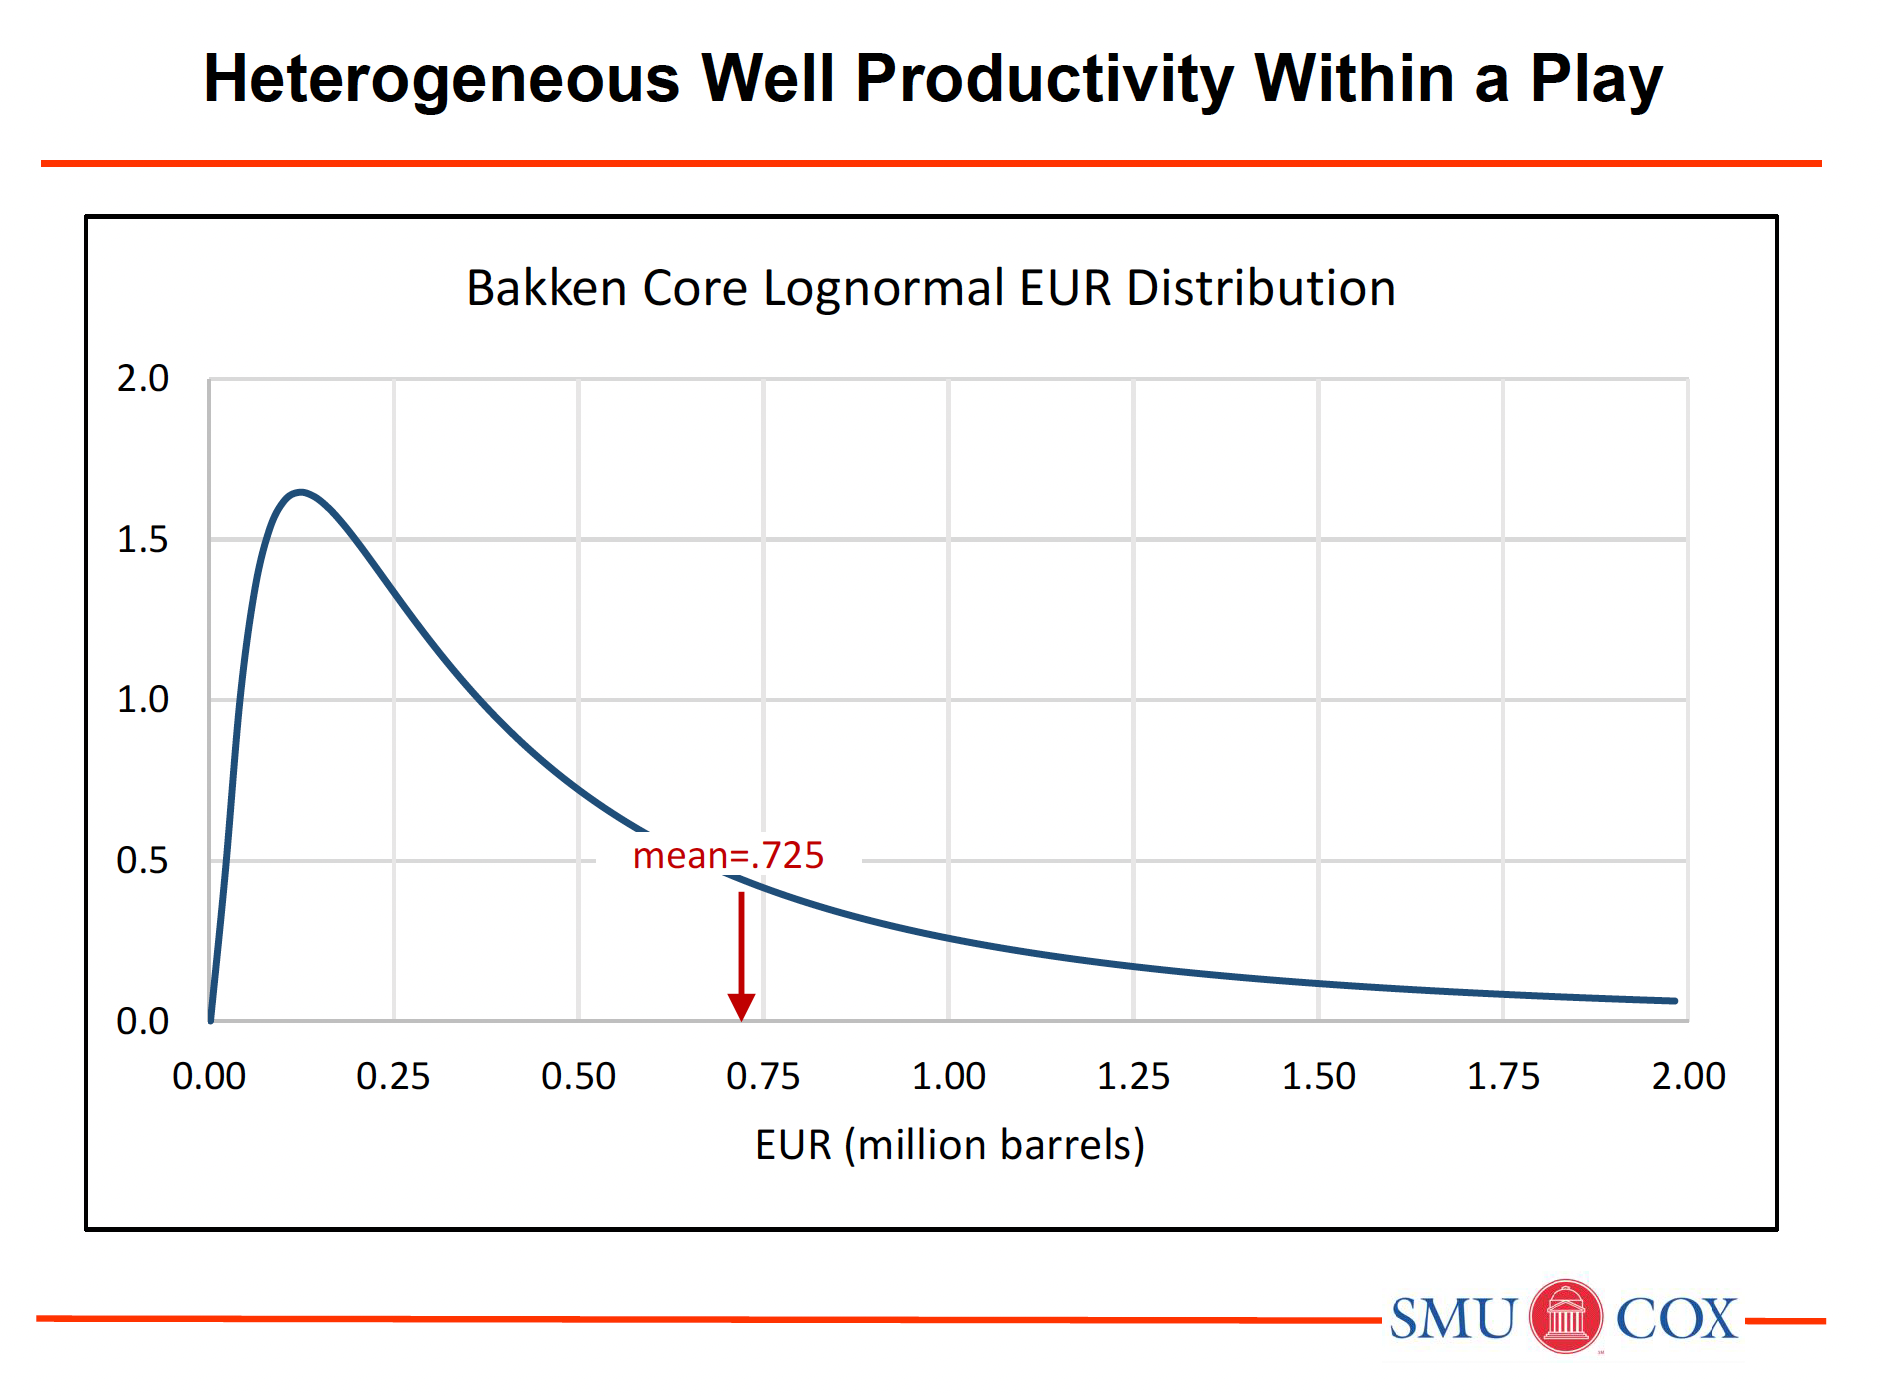
\includegraphics[width=0.85\linewidth]{figures/smith2016_slide4.png}
\caption*{\citet{smith2016}, slide 4 of the EIA Energy Finance Workshop deck.
Lognormal estimated ultimate recovery (EUR) distributions by US shale
play.}
\label{fig:smith2016-slide4}
\end{figure}

\begin{figure}[H]
\centering
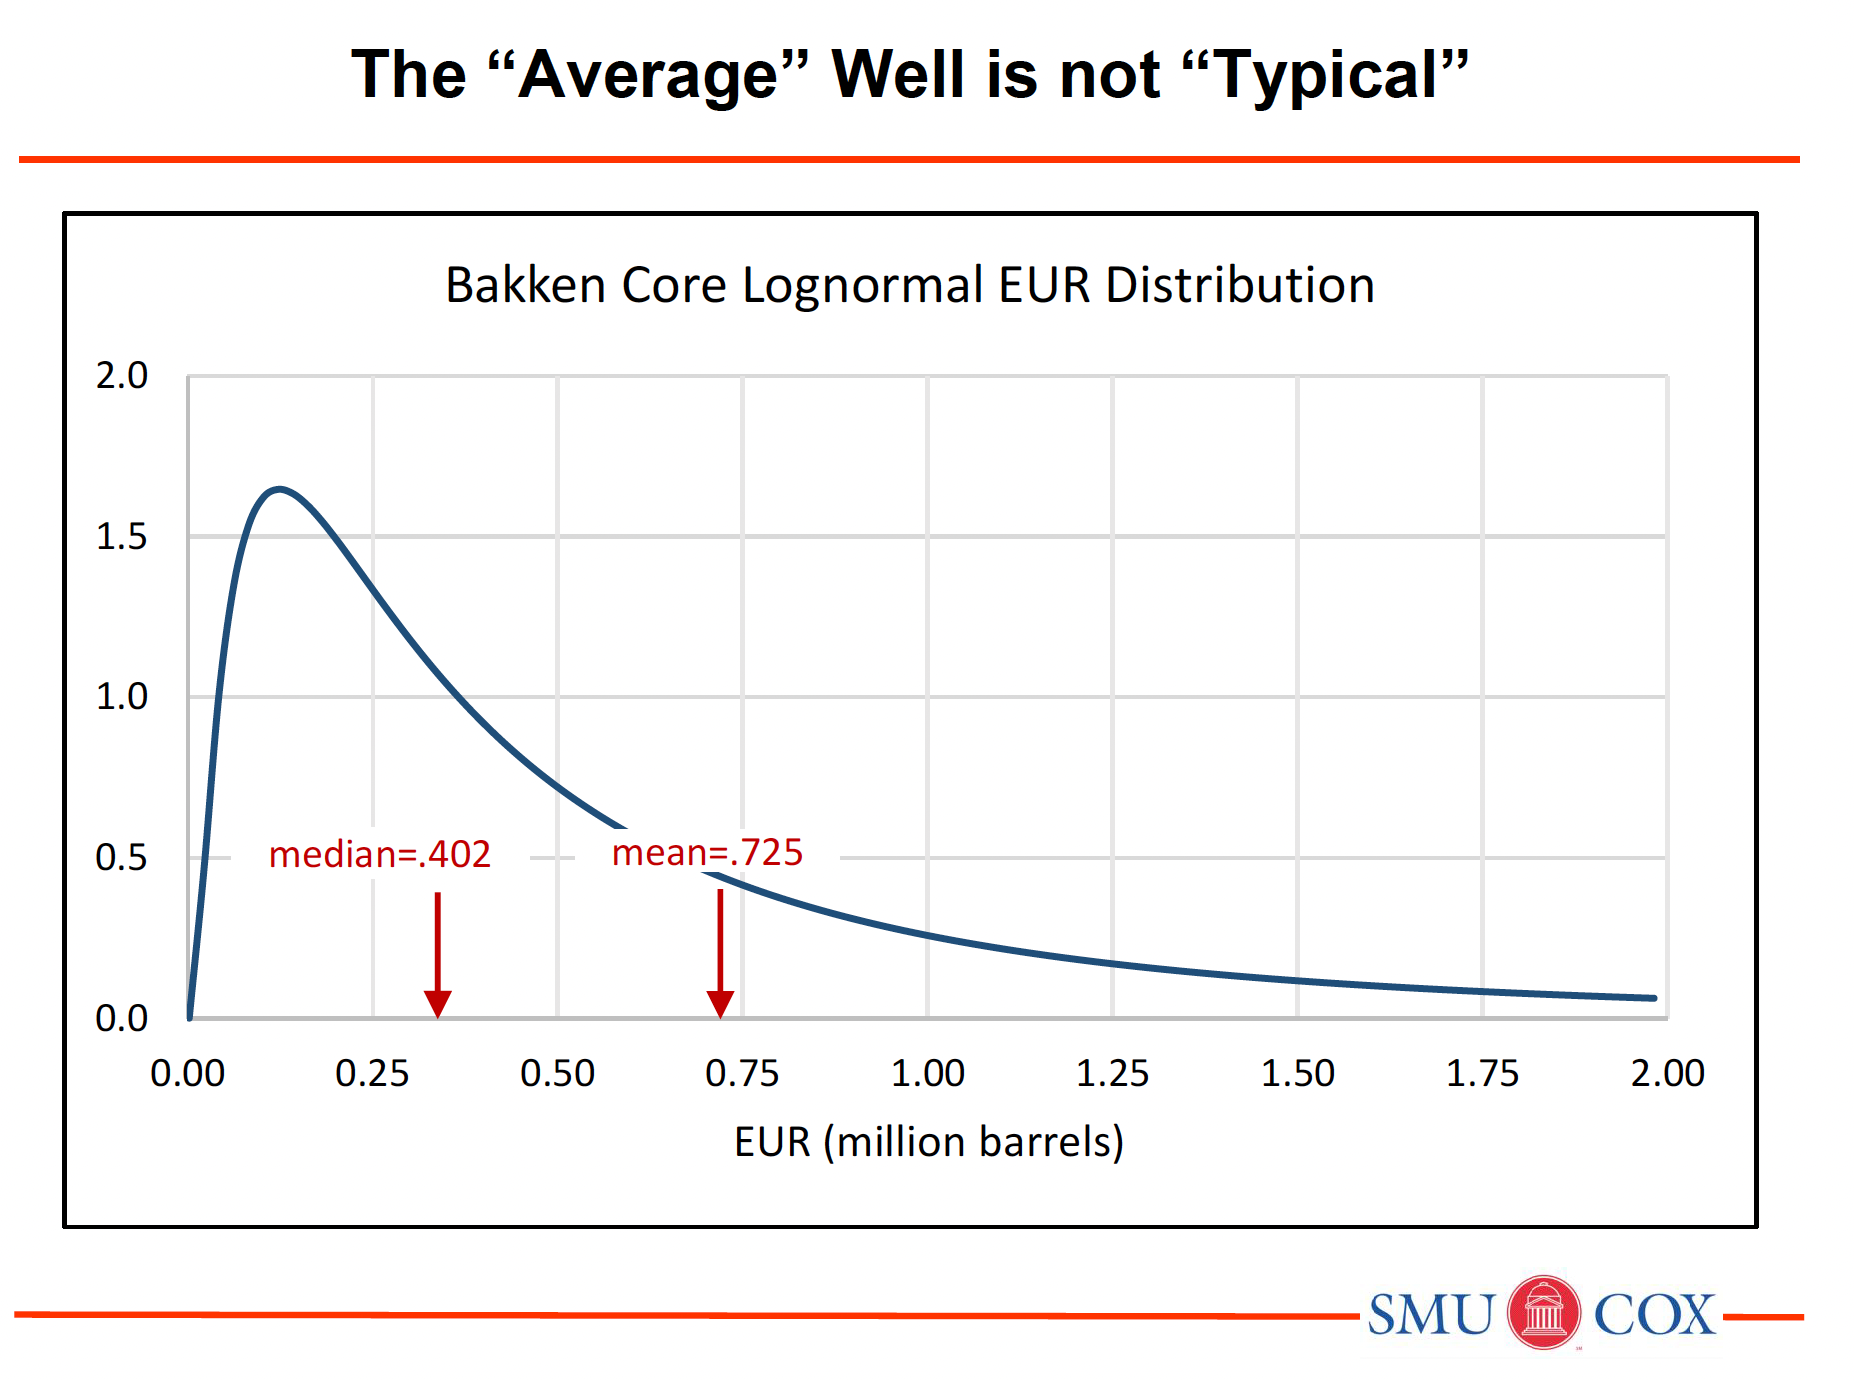
\includegraphics[width=0.85\linewidth]{figures/smith2016_slide5.png}
\caption*{\citet{smith2016}, slide 5. Continued lognormal EUR distributions.}
\label{fig:smith2016-slide5}
\end{figure}

\begin{figure}[H]
\centering
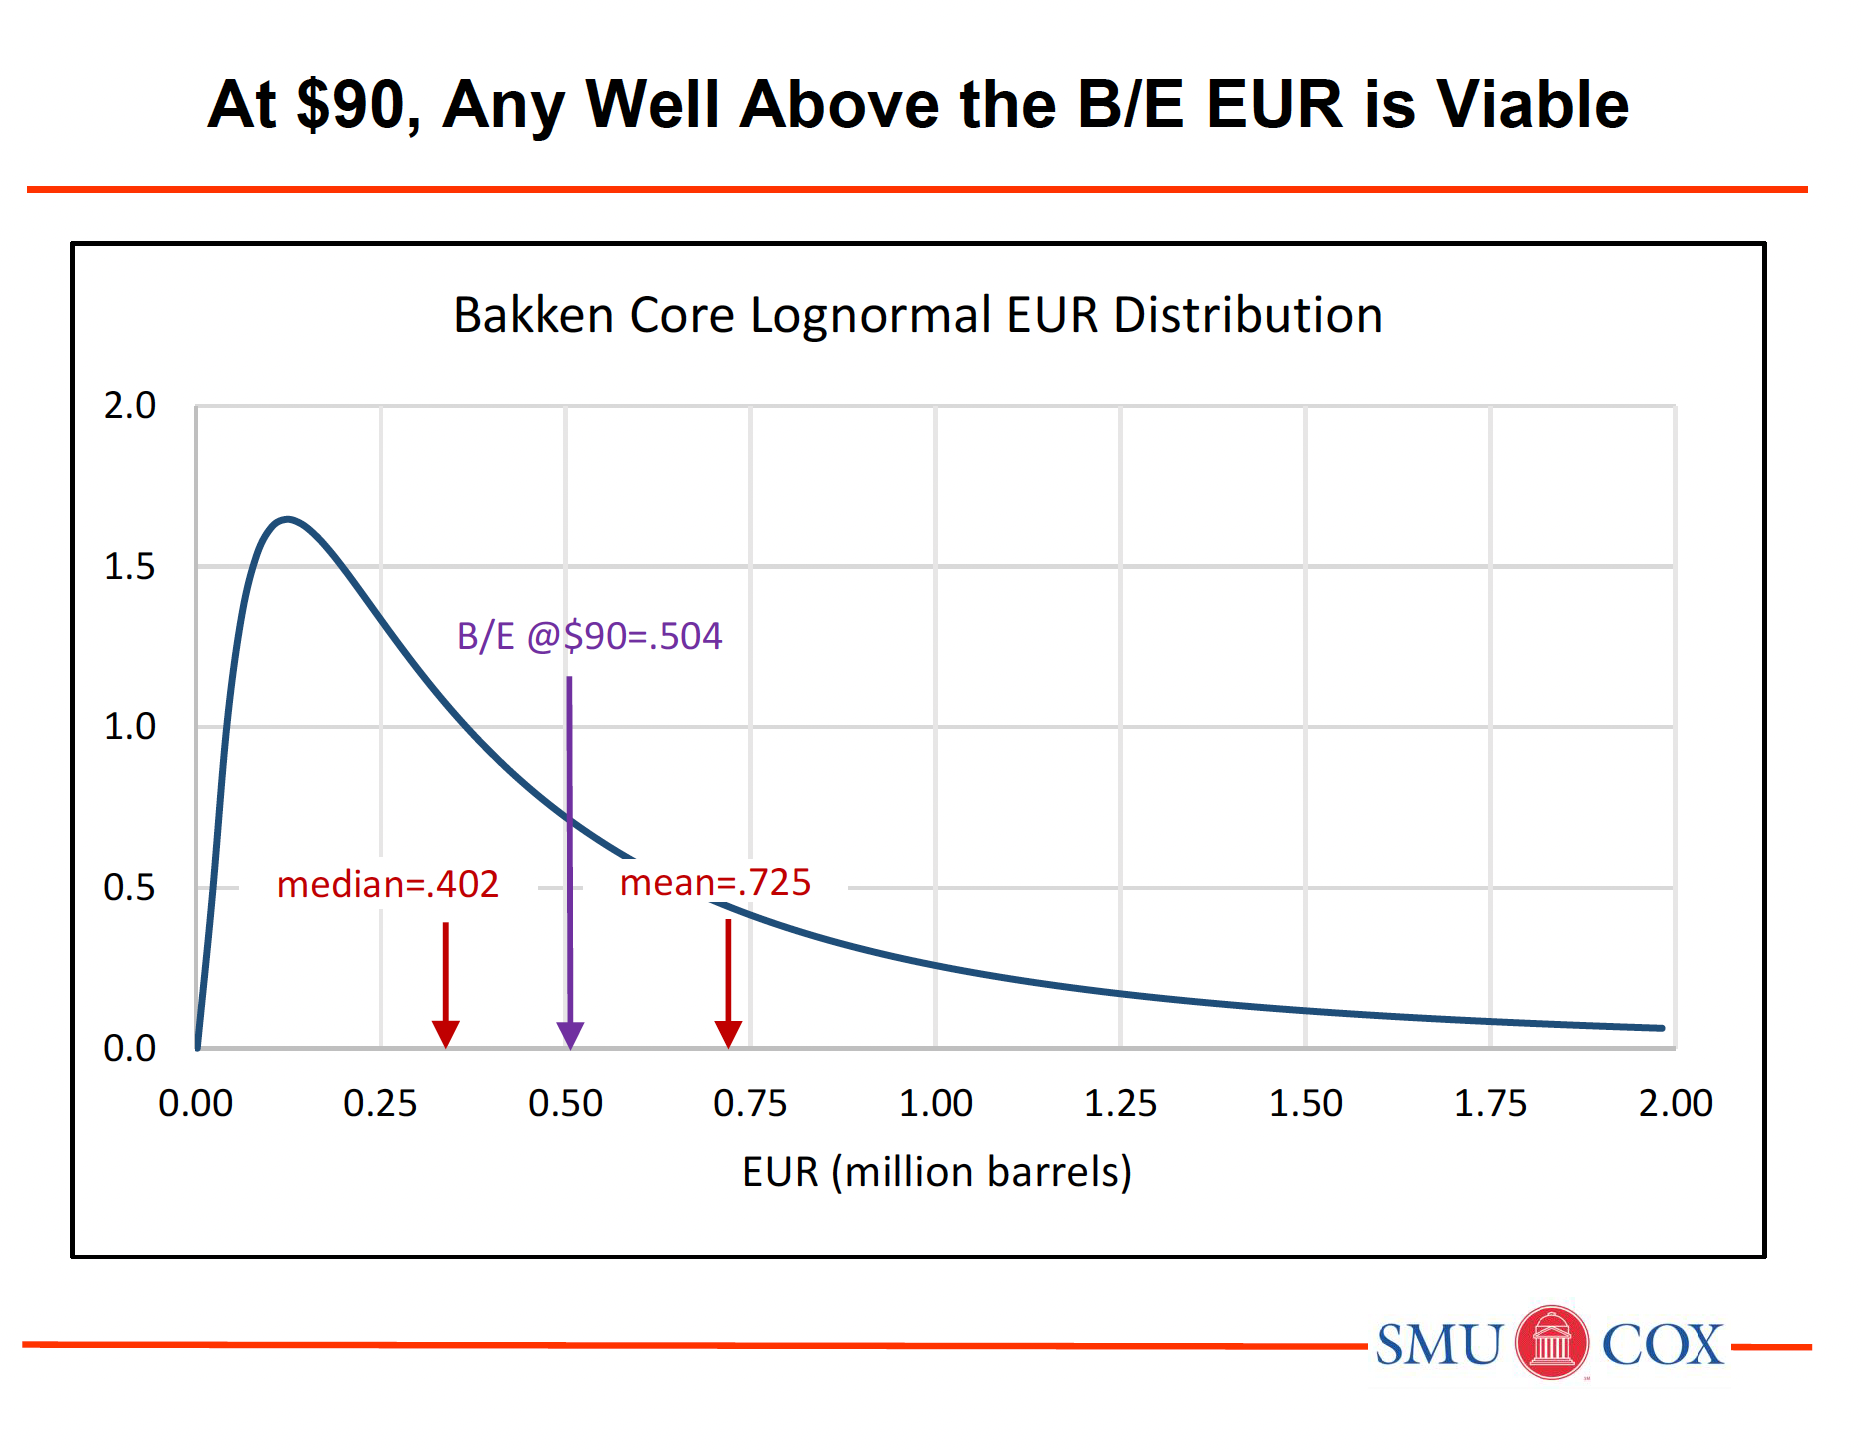
\includegraphics[width=0.85\linewidth]{figures/smith2016_slide6.png}
\caption*{\citet{smith2016}, slide 6. Distributional summary by major play.}
\label{fig:smith2016-slide6}
\end{figure}

\clearpage
\section{\texorpdfstring{\citet{till2016}}{Till (2016)}: OPEC spare capacity and convex price response}
\label{app:till}
\setcounter{figure}{0}

\begin{figure}[H]
\centering
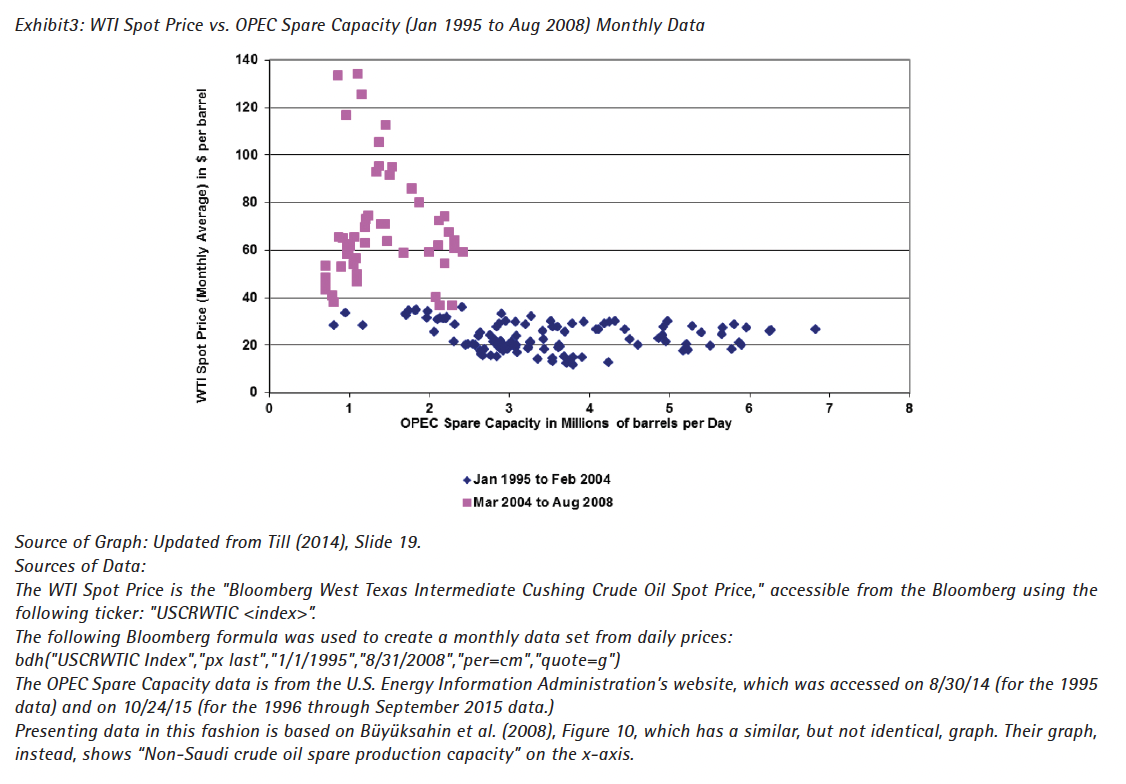
\includegraphics[width=0.9\linewidth]{figures/till2016_exhibit3.png}
\caption*{\citet{till2016}, Exhibit~3. Scatter of OPEC spare capacity against
the WTI price, illustrating the convexity that emerges below the
$2$~mbd spare-capacity threshold.}
\label{fig:till2016}
\end{figure}

\clearpage
\section{\texorpdfstring{\citet{huppmann2013}}{Huppmann (2013)}: OPEC market-power trajectories}
\label{app:huppmann}
\setcounter{figure}{0}

\begin{figure}[H]
\centering
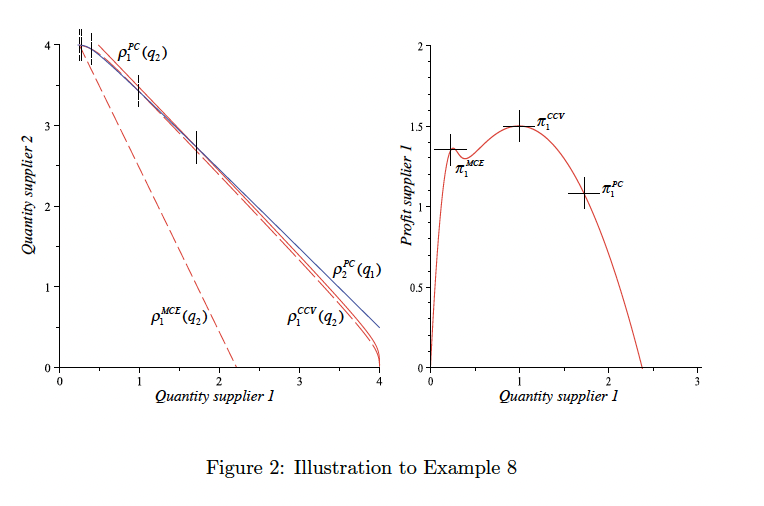
\includegraphics[width=0.8\linewidth]{figures/huppmann2013_fig2.png}
\caption*{\citet{huppmann2013}, Figure~2. OPEC market-power trajectories,
2003-2011.}
\label{fig:huppmann2013-fig2}
\end{figure}

\begin{figure}[H]
\centering
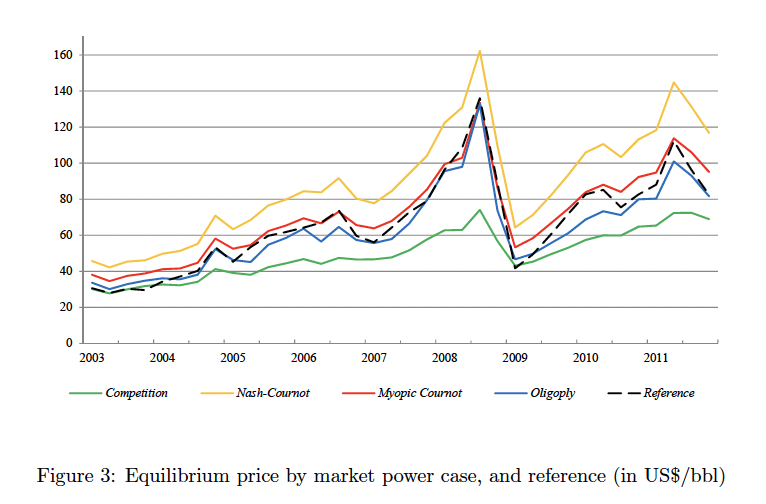
\includegraphics[width=0.8\linewidth]{figures/huppmann2013_fig3.png}
\caption*{\citet{huppmann2013}, Figure~3. OPEC market-power trajectories,
2003-2011.}
\label{fig:huppmann2013-fig3}
\end{figure}

\clearpage
\section{\texorpdfstring{\citet{almutairi2025}}{Almutairi et al. (2025)}: Counterfactual oil-price volatility}
\label{app:almutairi}
\setcounter{figure}{0}
\setcounter{table}{0}

\begin{table}[H]
\centering
\caption*{\citet{almutairi2025}, Table~3. Historical versus
counterfactual oil-price volatility for the Pandemic and Ukraine War
episodes.}
\label{tab:almutairi2025}
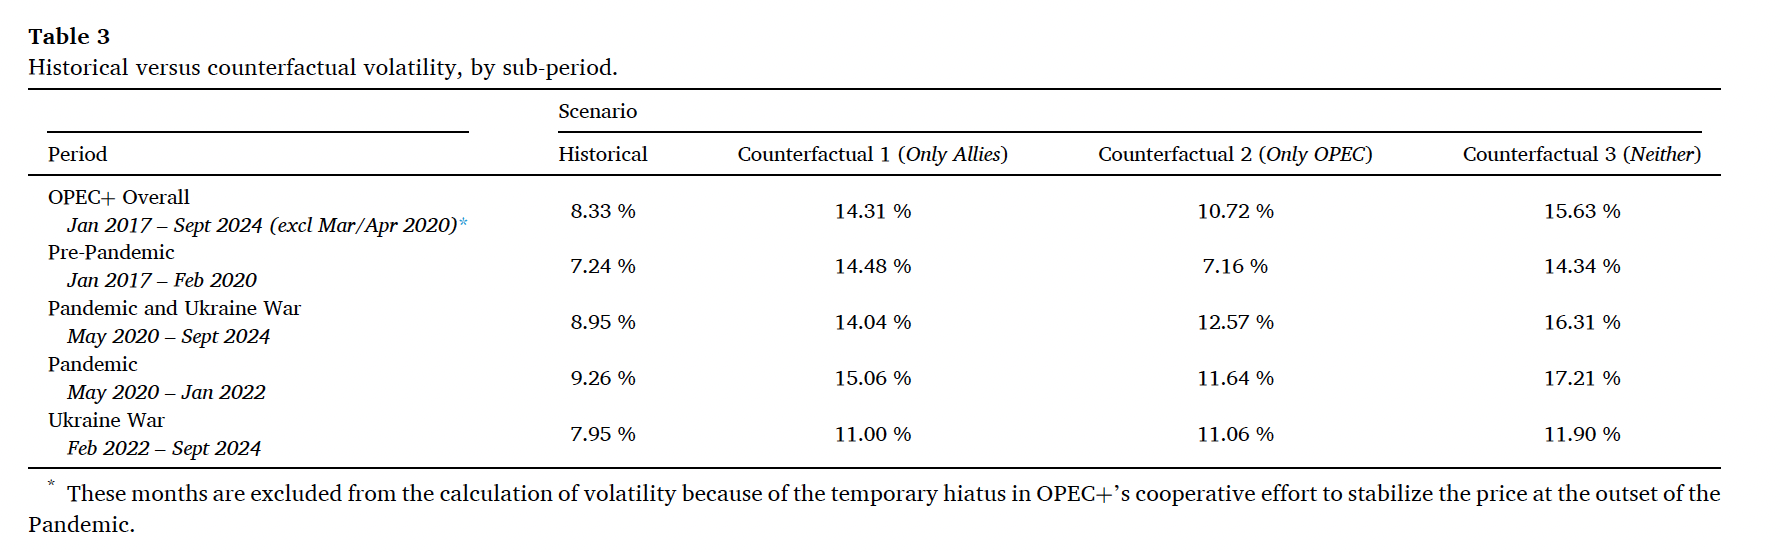
\includegraphics[width=\linewidth]{figures/almutairi2025_table3.png}
\end{table}

\begin{figure}[H]
\centering
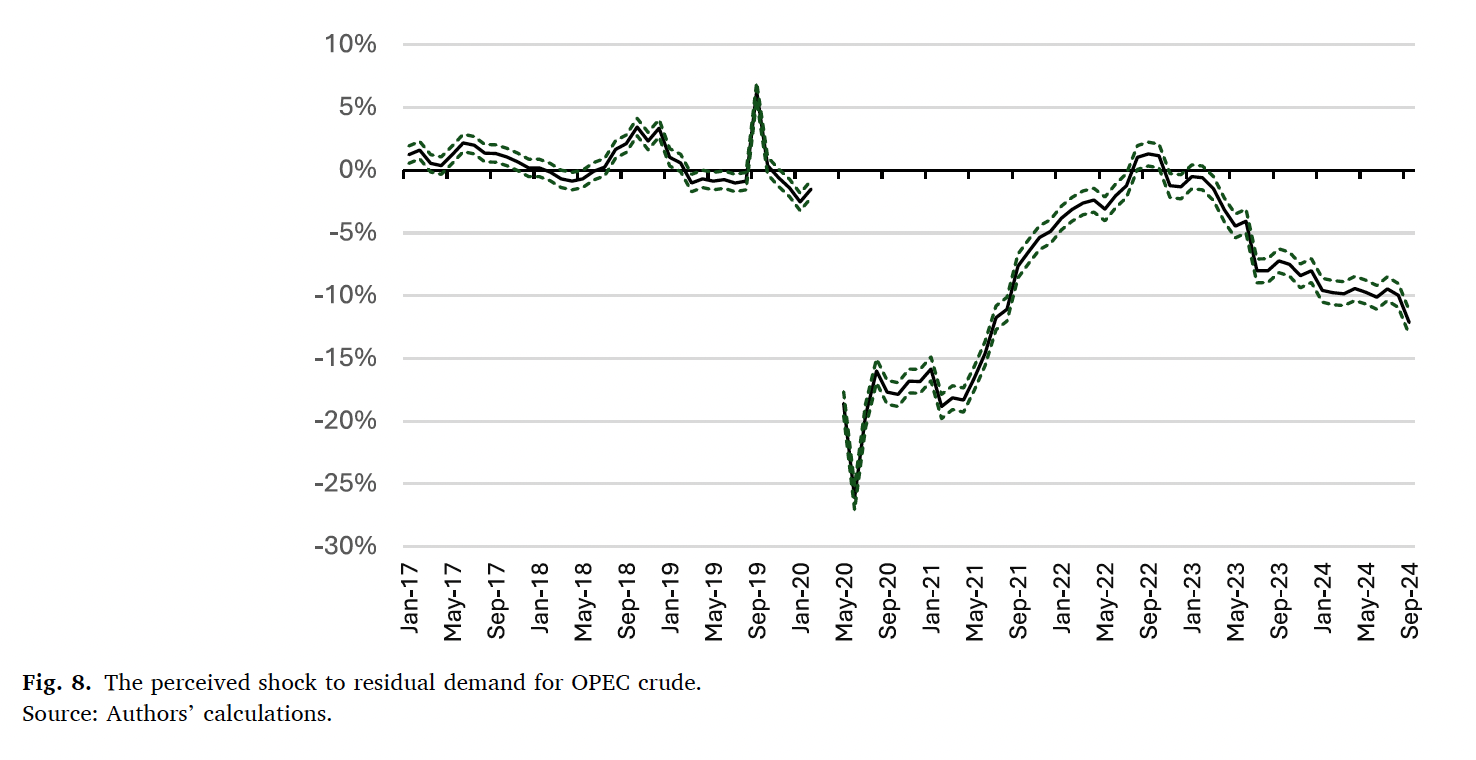
\includegraphics[width=\linewidth]{figures/almutairi2025_fig8.png}
\caption*{\citet{almutairi2025}, Figure~8. Perceived shock
to residual demand for OPEC crude underlying the counterfactual exercise.}
\label{fig:almutairi2025-fig8}
\end{figure}

\clearpage
\section{\texorpdfstring{\citet{almoguera2011}}{Almoguera et al. (2011)}: Regime-switching probabilities}
\label{app:almoguera}
\setcounter{figure}{0}
\setcounter{table}{0}

\begin{table}[H]
\centering
\caption*{\citet{almoguera2011}, Table~3. Regime-switching
probabilities between collusive and Cournot phases for OPEC, 1974-2004.}
\label{tab:almoguera2011}
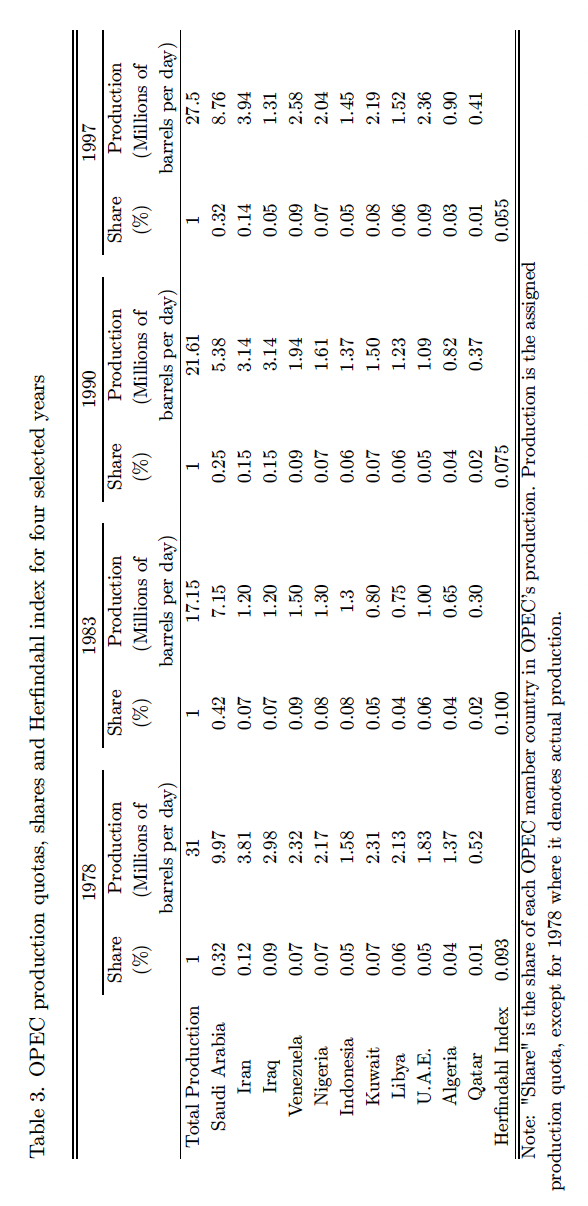
\includegraphics[width=0.55\linewidth]{figures/almoguera2011_table3.png}
\end{table}

\clearpage
\section{\texorpdfstring{\citet{beharritz2017}}{Behar and Ritz (2017)}: Market-share regime thresholds}
\label{app:behar-ritz}
\setcounter{figure}{0}

\begin{figure}[H]
\centering
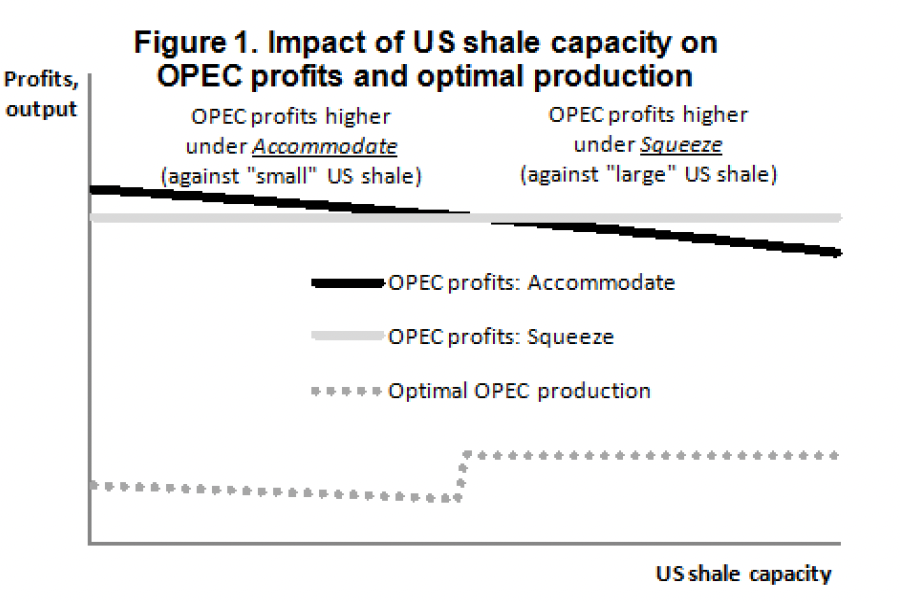
\includegraphics[width=0.9\linewidth]{figures/behar_ritz2017_fig4.png}
\caption*{\citet{beharritz2017}, Figure~4. Accommodation vs.\
market-share regime thresholds in the swing-producer model.}
\label{fig:behar-ritz2017}
\end{figure}

